\chapauthor{Гулякина Н.А.\\Козлова Е.И.\\Гракова Н.В.\\Оськин А.Ф.\\Головатый А.И.\\Самодумкин С.А.\\Ли В.}
\chapter{Автоматизация образовательной деятельности в рамках Экосистемы OSTIS}
\chapauthortoc{Гулякина Н.А.\\Козлова Е.И.\\Гракова Н.В.\\Оськин А.Ф.\\Головатый А.И.\\Самодумкин С.А.\\Ли В.}
\label{chapter_learning_systems}

\abstract{Аннотация к главе.}

\section{Общие принципы автоматизации образовательной деятельности с помощью ostis-систем}

Организация образовательной деятельности сегодня во многом определяет уровень развития любого государства и общества. Поэтому вполне объясним большой интерес к применению телекоммуникационных и компьютерных технологий в целях повышения эффективности этой деятельности. В этой связи особую актуальность приобретает такое направление исследований из области искусственного интеллекта, как интеллектуальные обучающие системы и автоматизация образовательной деятельности. Интеллектуальные обучающие системы (ИОС) должны стать частью комплекса подготовки специалиста. В то же время, такие системы можно эффективно использовать и в процессе обеспечения повышения квалификации, при осуществлении непрерывного образования. При этом одной из особенностей разработки интеллектуальных обучающих систем становится то, что пользователями таких систем будут и неспециалисты в области компьютерных и телекоммуникационных технологий, люди, существенно разные и по возрасту, и по уровню знаний в той или иной предметной области. Это является стимулом для развития технологий искусственного интеллекта в различных прикладных областях деятельности человека для реализации возможности построения ИОС для подготовки специалистов разных профессиональных направлений. Наиболее перспективным с точки зрения разработки и внедрения ИОС в учебный процесс ВУЗов видится использование экосистемы OSTIS для формирования как элементов обучающих и образовательных систем, так и их интеграции в единые комплекс.

В связи с развитием средств компьютерной поддержки процесса обучения и создания автоматизированных обучающих систем и систем дистанционного обучения, появилась острая необходимость в интеллектуализации всего процесса обучения, так как традиционные системы уже не в силах удовлетворить всех потребностей, как учащихся, так и преподавателей. Это произошло отчасти и потому, что автоматизированные обучающие системы предполагали лишь наличие разветвленной системы ссылок, предлагая обучаемому самому, вне зависимости от его уровня знаний, выбирать путь для дальнейшего обучения. Эффективность обучения определяется не только выбором среды обучения, но и формами представления знаний. Именно форма представления знаний играет важную роль в развитии дидактического принципа ``интеллектуальной наглядности'' среды обучения. К числу основных задач, направленных на интеллектуализацию компьютерных средств обучения (КСО) можно отнести ориентацию на семантическое представление используемых знаний (учебного материала, знаний об обучаемых, знаний о методах и технологиях обучения, знаний об учебных задачах, знаний об учебных лабораторных работах). Семантическое представление знаний позволяет, например, обеспечить достаточно эффективную компьютерную реализацию такой формы обучения, как консультация обучаемого по заданному предмету.

Современные КСО должны обеспечивать структуризацию, систематизацию и интеграцию учебного материала, возможность навигации по семантическому пространству учебного материала и ассоциативный доступ к любому его фрагменту, а также адекватное и наглядное представление обучаемому семантической структуры этого материала. Необходимо сокращать время разработки КСО, используя технологии параллельного проектирования, в основе которой лежит разбиение учебного материала соответствующей учебной дисциплины на достаточно самостоятельные разделы, с последующей интеграцией в единую интегрированную интеллектуальную обучающую систему по всей дисциплине.

Главной задачей любой обучающей системы является предоставление пользователю информации об изучаемой дисциплине в понятном и наглядном виде. Решение этой задачи возлагается на электронный учебник, который является неотъемлемой частью любой компьютерной системы обучения. Электронный учебник представляет собой компьютерное средство обучения, ориентированное на самостоятельную работу обучаемого и обеспечивающее:

\begin{textitemize}
	\item хранение учебного материала в электронном виде;
	\item отображение учебного материала обучаемому;
	\item возможность навигации по учебному материалу;
	\item редактирование учебного материала (для разработчиков электронного учебника).
\end{textitemize}

Однако на современном этапе, когда объемы информации стремительно возрастают, появляется необходимость в разработке таких электронных учебников, которые бы обеспечивали:

\begin{textitemize}
	\item возможность семантической структуризации учебного материала;
	\item интеграцию различных форм представления учебного материала;
	\item ассоциативный доступ к фрагментам учебного материала;
	\item возможность интеграции учебной информации с учебно-методической информацией;
	\item возможность интеграции самих электронных учебников.
\end{textitemize}

Одним из подходов к решению задачи представления и обработки знаний в КСО является использование графодинамических моделей обработки знаний, представленных однородными семантическими сетями с базовой теоретико-множественной интерпретацией. Особенностями таких моделей являются:

\begin{textitemize}
	\item приспособленость к распределенной, асинхронной и параллельной обработке знаний;
	\item наглядная визуализация сложноструктурированных знаний и метазнаний;
	\item интеграция семантического представления знаний с любыми другими формами представления информации;
	\item интегрируемость различных механизмов обработки знаний.
\end{textitemize}

Семантический электронный учебник является тем КСО, которое имеет более развитые средства отображения семантической структуры предметной области с соответствующими навигационными возможностями.

Существенное отличие семантического электронного учебника от традиционного электронного учебника состоит в представлении учебного материала на семантическом уровне. В результате этого, с практической точки зрения, усиливаются возможности электронного учебника как обучающей среды, появляется возможность эффективного самостоятельного изучения предмета.

\textbf{\textit{семантический электронный учебник}} -- это электронный учебник, в основе которого лежит представление учебного материала в виде гипермедийной семантической сети [4] и обеспечивается возможность семантической навигации и ассоциативного доступа к любому фрагменту учебного материала.

Учебная база знаний семантического электронного учебника представляет собой гипермедийную семантическую сеть, структурирующую учебный материал. В виде гипермедийной семантической сети представляется вся учебная информация, такая как, тематические планы обучения, содержательная структура учебного материала, непосредственно сам учебный материал. Основным преимуществом такой формы представления учебной информации является, во-первых, приспособленность семантических сетей для представления неформальных предложений естественного языка, во-вторых, обеспечение наглядности такого представлениями.

Формирование учебных материалов семантического электронного учебника происходит путем формализации знаний предметной области и описания их на соответствующих языках представления знаний, а также с использованием различных традиционных технологий представления информации. Технология разработки гипермедийных семантических сетей является результатом интеграции традиционных гипермедийных технологий, мультимедиа-технологий, а также технологий, связанных с представлением структуры знаний в виде семантических сетей.

Основным языком представления знаний для семантического электронного учебника является базовый семантический язык SC (Semantic Code), который является ядром открытого семейства графовых языков представления знаний, построенных на теоретико-множественной основе. Главным достоинством языка SC является то, что он представляет собой удобную основу для создания целого семейства языков, имеющих различное назначение и легко интегрируемых друг с другом.

Для навигации по семантическому пространству учебного и учебно-методического материала семантического электронного учебника разработаны следующие операции:

\begin{textitemize}
	\item навигационно-поисковые операции для баз знаний, представленных на языке SC;
	\item операции поиска заданного фрагмента учебного материала;
	\item операции поиска понятий;
	\item операции поиска учебных вопросов и задач.
\end{textitemize}

При интеграции семантических электронных учебников решаются следующие проблемы:

\begin{textitemize}
	\item поиск противоречий;
	\item выявление пар синонимичных элементов;
	\item локализация предположительно синонимичных пар элементов.
\end{textitemize}

Семантические электронные учебники представляют собой принципиально новый тип электронных учебников, в которых явно (в визуальной форме) представлена семантическая структура учебного материала. В семантических электронных учебниках полностью сохраняется преемственность с традиционными формами представления учебного материала. К достоинствам семантических учебников можно отнести:

\begin{textitemize}
	\item
	обеспечение семантической структуризации учебного материала;
	\item
	возможность семантической навигации по учебному материалу с помощью навигационно-поисковой графодинамической ассоциативной машины;
	\item
	простые механизмы интеграции семантических электронных учебников, в основе которых лежит явное описание междисциплинарных связей, позволяет разрабатывать электронные учебники по комплексу смежных учебных дисциплин.
\end{textitemize}

Этапы преобразования традиционного учебника в семантический электронный учебник:

\textbf{1 этап.} Описание структуры исходного учебного материала и библиографических атрибутов.

\textbf{2 этап.} Разбиение текста традиционного учебника на семантически элементарные фрагменты с указанием последовательности этих фрагментов в исходном тексте.

\textbf{3 этап.} Установление семантической типологии выделенных элементарных фрагментов текста.

\textbf{4 этап.} Выделение в указанных текстовых фрагментах ключевых понятий и формирование соответствующих им sc-узлов, а также указание связей соответствующих фрагментов с указанными sc-узлами.

\textbf{5 этап.} Перевод на язык SC указанных выделенных фрагментов исходного учебного материала. Установление связей семантической эквивалентности между исходными текстовыми фрагментами и их формализованной записью на языке SC.

\textbf{6 этап.} Построение определений или пояснений указанных выше ключевых понятий (если таковые отсутствуют в учебнике), а также ключевых узлов, которые введены для описания структуры предметной области на русском языке и языке SC, с установлением связи семантической эквивалентности текстов между ними. Кроме того, на данном этапе для выделенного набора понятий и отношений предметной области необходимо отобрать и сформулировать их основные определения, комментарии к ним, расшифровать их семантику и выделить группы семантически связанных элементов предметной области.

\textbf{7 этап.} Построение теоретико-множественной классификационной схемы выделенных понятий.

\textbf{8 этап.} Указание синонимов и омонимов выделенных понятий.

\textbf{9 этап.} Описание наиболее важных соотношений между указанными понятиями (кроме указанной выше теоретико-множественной классификации понятий).

Технологически семантический электронный учебник можно построить полностью сохраняя традиционный учебник, лишь надстраивая над ним соответствующую семантическую сеть. Это актуально на сегодняшний день, поскольку существует большое количество качественного учебно-методического материала, представленного в традиционной форме.

\section{Автоматизация среднего образования с помощью ostis-систем}

Современный человек в информационном обществе обязан уметь адаптироваться к быстро меняющимся информационным потокам. Формирование таких навыков -- главная задача учебных организаций, к которым в современных условиях предъявляются все более высокие требования.

Дальнейшее развитие образования невозможно без совершенствования методов и средств его информатизации. Как и раньше существуют проблемы развития мотивированного отношения к обучению, формирования навыков самообучения, несогласованности учебных материалов. Для преодоления этих проблем существует острая необходимость в применении технологий искусственного интеллекта в процессе обучения, так как традиционные компьютерные системы обучения уже не в силах удовлетворить всем требованиям, как со стороны учащихся, так и со стороны преподавателей.

Очевидной становится проблема нехватки времени на образование. Для того, чтобы получить хотя бы базовые знания, человеку приходится обучаться в системах среднего и высшего образования в течение 11-18 лет, не считая дошкольного и последипломного образования. Кроме этого, темпы развития современного общества и, в частности, различных технологий, показывают, что каждому человеку для того, чтобы сохранять профессиональную пригодность и быть полноценным членом общества необходимо постоянно развиваться и обучаться.

Предлагаются следующие этапы работ по реализации предлагаемого комплексного инновационного проекта

\textbf{Проект 1.} Разработка семантических электронных учебников по основным дисциплинам школьного образования, имеющих средства редактирования, верификации, интеграции баз знаний, а также средства навигации по базе знаний.

\textbf{Проект 2.} Разработка интеллектуальных решателей задач для каждого семантического электронного учебника.

\textbf{Проект 3.} Разработка специальных средств пользовательских интерфейсов для каждого семантического электронного учебника.

\textbf{Проект 4.} Построение на базе разработанных семантических учебников интеллектуальных обучающих систем, осуществляющих управление обучением на основе индивидуальных особенностей обучаемого.

\textbf{Проект 5.} Разработка интегрированного комплекса обучающих систем, обеспечивающего комплексное обучение, соответствующее среднему образованию.

\textbf{Проект 6.} Разработка семантического ассоциативного компьютера (с не фон-неймановской архитектурой), ориентированного на обработку семантических сетей и обеспечивающего аппаратную поддержку разработанного комплекса обучающих систем.

Рассмотрим реализацию указанного подхода к разработке ИОС на примере ОИС по Геометрии Евклида.

Основой любой интеллектуальной системы является база знаний. Это наиболее динамичный компонент, который меняется в течение всего жизненного цикла. Поэтому сопровождение интеллектуальных систем --- серьезная проблема.

Наиболее важный параметр базы знаний --- качество содержащихся знаний. Лучшие базы знаний включают самую релевантную и актуальную информацию, имеют совершенные системы поиска информации и тщательно продуманную структуру и формат знаний. Поэтому стадия концептуального анализа или структурирования знаний традиционно является ``узким местом'' в жизненном цикле разработки интеллектуальных систем. Из этого следует, что разработчиками баз знаний может быть ограниченный круг специалистов, что не позволяет массово разрабатывать качественные интеллектуальные системы.

Интеллектуальная справочная система по геометрии разработана на основании технологии проектирования интеллектуальных систем OSTIS (Open Semantic Technology for Intelligent Systems).

Применим методику проектирования баз знаний, основанную на технологии OSTIS, при проектировании базы знаний интеллектуальной справочной системы по геометрии.

Согласно методике, первым этапом проектирования баз знаний является разработка первой версии тестового сборника предполагает выделение семантически полного набора вопросов, ответы на которые должны содержаться в стартовой версии базы знаний. Для системы по геометрии были выделены следующие классы вопросов: запросы определений; запросы основных свойств заданного объекта; запрос доказательств высказываний; запросы минимального высказывания (минимального фрагмента базы знаний), описывающего семантически значимую связь между всеми объектами заданного множества объектов; запросы пар высказываний, описывающих отличающиеся свойства заданных двух объектов и др.

На следующем этапе проектирования необходимо записать ответы на выделенные вопросы, тем самым будет формироваться стартовая версия базы знаний. В процессе записи ответов на вопросы на формальном языке SCg выделяются ключевые узлы описываемой предметной области. К ключевым узлам, являющимися классами объектов исследования геометрии, относятся следующие ключевые узлы: геометрическая фигура, точка, отрезок, луч, линия, плоскость, многоугольник, треугольник, четырехугольник и др. К ключевым узлам, являющимися отношениями и составляющими предмет исследования, относятся: параллельность, перпендикулярность, пересечение, конгруэнтность, сторона, внутренний угол, лежать между, лежать против, вписанность и др.

На следующем этапе проектирования каждый выделенный ключевой узел геометрии анализируется на предмет его свойств и описывается в псевдоестественной форме с использованием специализированного языка SСn-кода (Semantic Code natural). Данная форма представления является промежуточной между представлением на естественном языке и формальном, и в дальнейшем она будет использоваться в качестве исходных данных для автоматической трансляции конструкций в формальное представление.

База знаний по геометрии на SCn-коде представляет собой семантически структурированный гипертекст. Все понятия из предметной области Геометрии имеют связи между собой, связи реализуются в виде ссылок, что позволяет переходить от понятия к понятию по определенной связи, указываемой при помощи ключевого слова SCn-кода.

В зависимости от типа описываемого понятия, статьи описания делятся на различные виды. В интеллектуальной справочной системе по геометрии были выделены следующие типы статей описания:

\textbf{\textit{формальная теория}} (пример описываемой сущности -- \textit{Геометрия Евклида})

\begin{textitemize}
	\item синонимичные названия теории;
	\item объект исследования;
	\item предмет исследования;
	\item декомпозиция на разделы;
	\item надтеория;
	\item система аксиом, лежащих в основе теории;
	\item неопределяемые понятия;
	\item противоречивые теории.
\end{textitemize}

\textbf{\textit{персона}} (пример описываемой сущности -- \textit{Евклид})

\begin{textitemize}
	\item годы жизни;
	\item место рождения и жизни;
	\item объект, автором чего персона является;
	\item учителя и ученики персоны;
	\item биография.
\end{textitemize}

\textbf{\textit{понятие, не являющееся отношением}} (примеры понятий -- \textit{отрезок}, \textit{треугольник}, \textit{многоугольник})

\begin{textitemize}
	\item синонимы понятия;
	\item классификация понятия по различным признакам;
	\item надклассы понятия и подклассы понятия;
	\item отношения, заданные на понятии;
	\item определение, пояснение понятия;
	\item понятия, на основе которых определяется указанное понятие;
	\item основные утверждения, описывающие свойства понятия;
	\item аналоги понятия и антиподы понятия.
\end{textitemize}

\textbf{\textit{отношение}} (примеры понятий -- \textit{внутренний угол*}, \textit{площадь*}, \textit{периметр*}, \textit{граничная точка*}, \textit{быть между\scnrolesign})

\begin{textitemize}
	\item синонимичные названия отношения;
	\item область определения отношения;
	\item схема отношения;
	\item домены отношения;
	\item классы отношения по признакам классификации:
	\begin{textitemize}
		\item арность
		\item ориентированность
		\item наличие кратных связок и встречных связок
		\item наличие мультисвязок
		\item транзитивность, рефлексивность
	\end{textitemize}
	\item подклассы отношения;
	\item аналоги отношения;
	\item утверждения, описывающие свойства данного отношения или его подмножеств.
\end{textitemize}

\textbf{\textit{высказывание}} (пример описываемой сущности -- \textit{Теорема Пифагора})

\begin{textitemize}
	\item в состав какой теории входит высказывание;
	\item логический статус (определение, аксиома, теорема);
	\item формулировка высказывания;
	\item логический тип (существование, несуществование, единственность, всеобщность, эвивалентность, необходимость и достаточность)
	\item на основании каких высказываний доказывается указанное высказывание;
	\item доказательство.
\end{textitemize}

\textbf{\textit{конкретный объект исследования}} (пример -- \textit{Треугольник ABC})

\begin{textitemize}
	\item идентификаторы объекта;
	\item рисунок;
	\item описание связей с другими фигурами и точками (стороны, вершины, биссектрисы, медианы, высоты, граница, точки пересечения и др.);
	\item числовые характеристики (периметр, площадь, величина углов, величина сторон и др.);
	\item типология по различным признакам.
\end{textitemize}

Таким образом, в базе знаний хранится большое многообразие видов знаний -- классы геометрических фигур (планарные фигуры, линейные фигуры, фигуры, имеющие граничные точки), конкретные фигуры (треугольник, трапеция, окружность), классы отношений, конкретные отношения, утверждения различного типа (аксиомы, теоремы, утверждения определяющего типа), доказательства утверждений (доказательства теорем, лемм), алгоритмы решения задач (в т.ч. геометрических построений), изображения, иллюстрирующие различные геометрические чертежи, видео, флеш, иллюстрирующие решение задач и различные геометрические построения. Возможность представления знаний различного вида позволяет описывать информацию в базе знаний с различных ракурсов, что в свою очередь переводит базу знаний на другой, более высокий интеллектуальный уровень.

Технология проектирования интеллектуальных решателей задач основана на задачно-ориентированной методологии. В связи с этим проектирование системы операций состоит из четырех основных этапов:

\begin{textitemize}
	\item создание тестового сборника задач, которые решаются в рамках исследуемой предметной области;
	\item определение списка операций, которые будут использоваться при решении задач из тестового сборника;
	\item создание семантической спецификации каждой из операций;
	\item реализация и отладка операций.
\end{textitemize}

Такая методика проектирования операций позволяет создавать предметно независимые операции для решения конкретных прикладных задач из исследуемой предметной области. Спроектированные таким образом операции являются переносимыми ip-компонентами (компонентами интеллектуальной собственности, от англ. intellectual property) и могут быть использованы в других интеллектуальных справочных системах.

Опишем этапы проектирования системы операций для интеллектуального решателя задач по геометрии на примере конкретной прикладной задачи.

Пусть дан некоторый плоский треугольник с известными длинами сторон. Необходимо найти величину площади заданного треугольника. С точки зрения геометрии задача является довольно тривиальной, однако ее решение будет достаточно непростым, если предположить, что пользователь не определился, что он хочет найти в треугольнике: площадь, углы, периметр или другие характеристики. При помощи sc-технологии {[}2{]} (sc -- semantic code), основанной на семантических сетях, можно универсально представить знания о данном треугольнике таким образом, чтобы все задачи, перечисленные выше, решались с помощью одного и того же набора операций.

Тестовый сборник задач будет состоять из единственной задачи, описанной выше.

Определим те операции, которые будут использованы при решении задачи о нахождении площади:

\begin{textitemize}
	\item операция поиска в базе знаний информации о значении искомой величины (площади) данного треугольника;
	\item операция поиска в базе знаний формулы, позволяющей по имеющейся информации найти значение искомой величины (площади);
	\item операция, осуществляющая прямой логический вывод (modus ponens);
	\item операция, которая осуществляет унификацию найденной (сгенерированной) формулы с учетом заданных параметров;
	\item операция, вычисляющая значение арифметического выражения;
	\item элементарные арифметические операции (сложение (вычитание), умножение (деление), возведение в степень (извлечение корня) и т.д.).
\end{textitemize}

Далее опишем часть третьего этапа проектирования на примере операции вычисления значения формулы.

\textbf{Пример семантической спецификации операции}

Семантическая спецификация операции -- это sc-конструкция, которая описывает интерфейс проектируемой операции (условие инициирования, название операции, возможные результаты работы).

Условием инициирования для этой операции является факт появле­ния в памяти sc-дуги, выходящей из узла ``запрос вычисления формулы''. После появления в памяти этой дуги вызывается операция ``calculation''. В результате работы этой операции либо вычисляется значение некоторой искомой величины, либо генерируются знания о том, что ответ не найден. Отрицательный результат работы этой операции может быть использован другими операциями для того, чтобы попытать­ся каким-либо другим способом вычислить значение искомой величины.

Завершающим этапом является реализация и тестирование спроектированной операции.

\begin{figure}[H]
	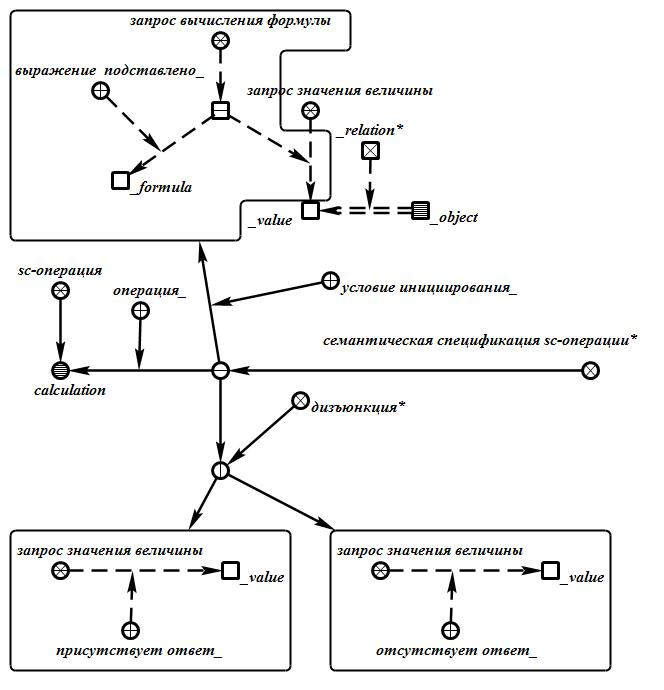
\includegraphics[scale=0.5]{images/part7/chapter_learning_systems/step1.jpg}
	\caption{Семантическая спецификация операции вычисления формулы}
	\label{fig:step1}
\end{figure}

Этап реализации также можно разбить на два шага:

\begin{textitemize}
	\item Разработка алгоритма операции
	\item Реализация программы на подходящем языке. Предпочтительно использовать специально адаптированный язык SCP (semantic code programming).
\end{textitemize}

SCP -- специальный язык программирования, предназначенный для обработки семантических сетей{[}3{]}.

Опишем алгоритм работы операции:

\begin{enumerate}
	\item
	Проверяем корректность структуры, которая представляет собой запрос.
	\item
	Из запроса получаем информацию об искомой величине.
	\item
	Находим узел, обозначающий искомую величину в формуле.
	\item
	Находим в формуле все связки отношений ``сложение*'', ``произведение*'' и ``возведение в степень*''.
	\item
	Просматриваем все связки, найденные в шаге 4.
	
	\begin{enumerate}
		\def\labelenumii{\arabic{enumii}.}
		\item
		Если связка принадлежит классу отношения ``сложение*'', то инициируем операцию сложения.
		\item
		Если связка принадлежит классу отношения ``произведение*'', то инициируем операцию умножения.
		\item
		Если связка принадлежит классу отношения ``возведение в степень*'', то инициируем операцию возведения в степень.
		\item
		Если количество выполняемых операций превысило определенный пользователем предел, то генерируем факт отсутствия ответа и завершаем работу операции.
	\end{enumerate}
	\item
	Если значение искомой величины не посчитано, то переходим к шагу 5.
	\item
	Генерируем факт присутствия ответа.
\end{enumerate}

\textbf{Пример протокола решения задачи}

Опишем протокол решения вышеописанной задачи. Протокол отражает последовательность запуска и выполнения операций, текущие условия их запуска, а также результаты выполнения каждой из операций.

\begin{enumerate}
	\item
	В памяти появляется конструкция вида:
\end{enumerate}

\begin{figure}[H]
	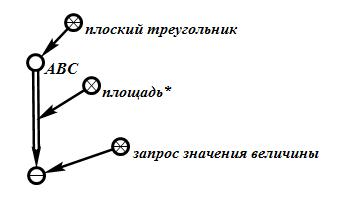
\includegraphics[scale=0.5]{images/part7/chapter_learning_systems/step2.jpg}
	\caption{Запрос значении площади треугольника АВС}
	\label{fig:step2}
\end{figure}

Запускаются операции find\_value и find\_formula, при этом выполнение find\_formula завершается, т.к. конструкция не полностью соответствует условиям запуска. find\_value проверяет наличие значения указанной величины и, не найдя его, заявляет о его отсутствии:

\begin{figure}[H]
	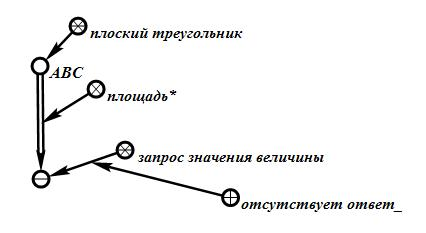
\includegraphics[scale=0.5]{images/part7/chapter_learning_systems/step3.jpg}
	\caption{Результат работы операции find\_value}
	\label{fig:step3}
\end{figure}

\begin{enumerate}
	\setcounter{enumi}{1}
	\item
	Снова запускаются операции find\_value и find\_formula, при этом выполнение find\_value завершается, т.к. конструкция не полностью соответствует условиям запуска.
\end{enumerate}

Операция find\_formula производит поиск в базе знаний подходящей формулы, которая позволила бы вычислить значение требуемой величины у указанного объекта. Под формулой понимается некоторое импликативное логическое высказывание, справедливое для произвольного класса объектов, которому принадлежит рассматриваемый объект (в данном случае -- треугольник), в посылке которого описаны требуемые для вычисления значения, а в заключении -- собственно арифметическое выражение, вычисление которого приводит к получению требуемого результата. В данном случае также используется сокращенная форма высказывания о всеобщности, т.е. по умолчанию квантором всеобщности связываются те переменные, которые присутствуют в обеих частях высказывания.

\begin{figure}[H]
	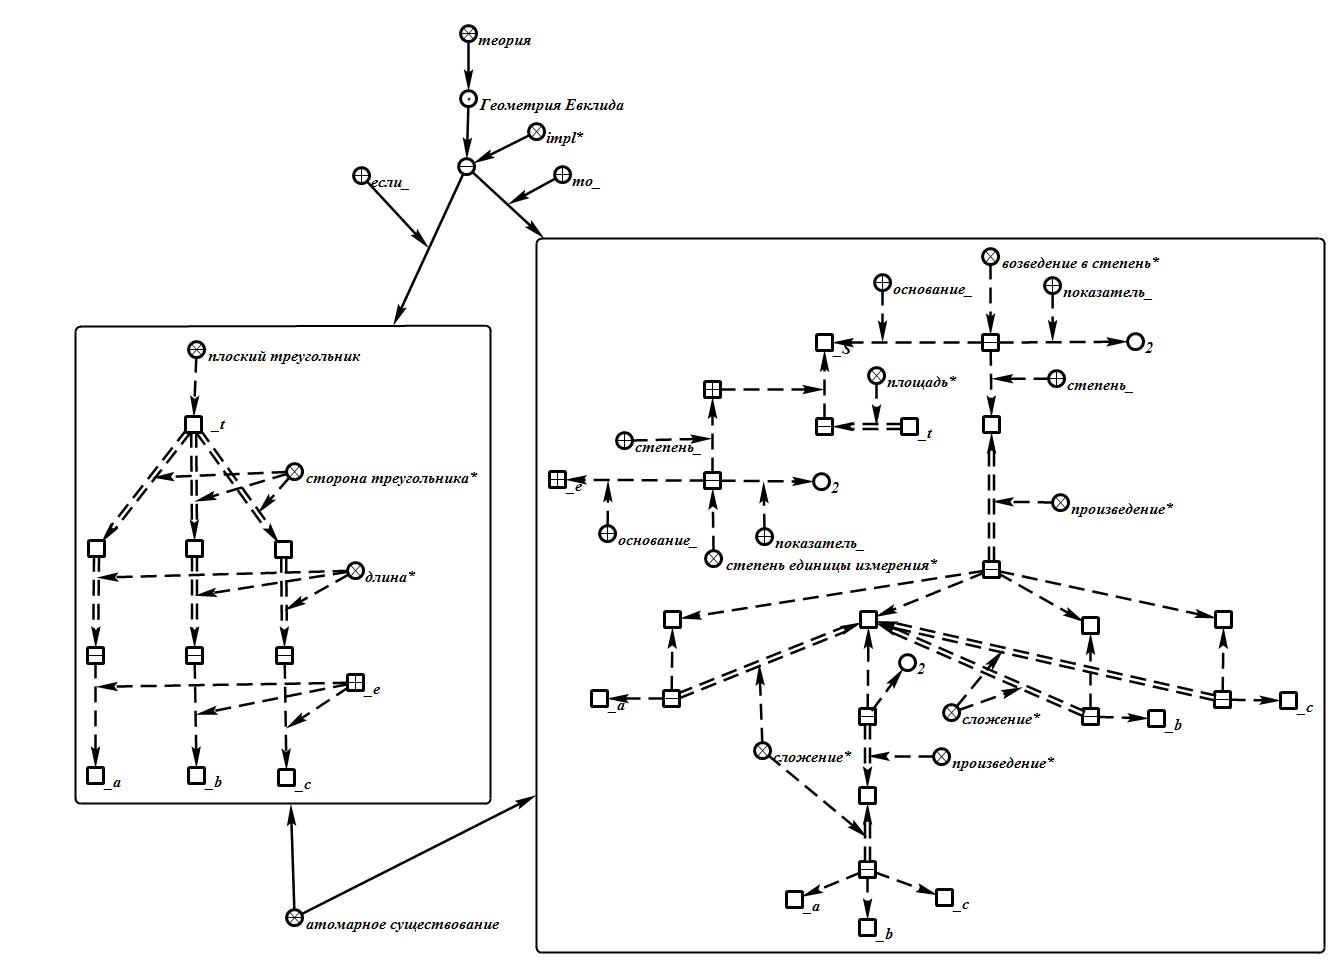
\includegraphics[scale=0.5]{images/part7/chapter_learning_systems/step4.jpg}
	\caption{Пример формулы -- формула Герона для вычисления площади треугольника}
	\label{fig:step4}
\end{figure}

При просмотре каждой из формул производится проверка на соответствие предполагаемого результата желаемому и проверка наличия в базе знаний всей необходимой информации. Например, в данном случае проверяется тот факт, что формула Герона позволяет вычислить именно площадь (а не периметр) треугольника (а не четырехугольника или круга). Далее проверяется тот факт, что в базе присутствуют длины всех трех сторон данного треугольника, что позволит воспользоваться именно формулой Герона. В противном случае перебор формул продолжается. В данном случае перебор формул заканчивается на формуле Герона. В памяти генерируется запрос на подстановку конкретных значений в формулу:

\begin{figure}[H]
	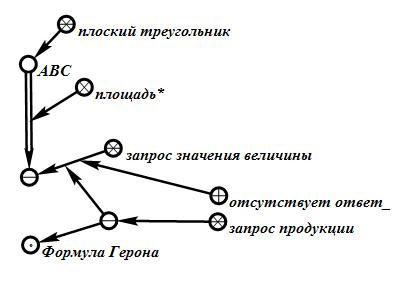
\includegraphics[scale=0.5]{images/part7/chapter_learning_systems/step5.jpg}
	\caption{Запрос на унификацию формулы}
	\label{fig:step5}
\end{figure}

\begin{enumerate}
	\setcounter{enumi}{2}
	\item
	Запускается операция find\_value\_production, задачей которой является унификация предложенной формулы константами из базы знаний. Операция использует посылку формулы для поиска значений, соответствующих именно указанному объекту (в данном случае -- длин треугольника АВС, а не какого-либо другого треугольника). После этого отбираются значения переменных, связанных квантором всеобщности, и производится генерация арифметического выражения с подстановкой в него значений связанных переменных из формулы. Результатом работы является константное арифметическое выражение, требующее вычисления, о чем сообщается путем генерации соответствующей конструкции.
	\item
	Далее запускается операция calculation, алгоритм и условия срабатывания которой подробно рассмотрены выше.
\end{enumerate}

В результате последовательного выполнения указанного набора операций у указанного объекта явно указывается значение требуемого параметра.

\section{Автоматизация высшего образования с помощью ostis-систем}

Можно выделить три основных направления интеллектуализации учебного процесса, соответствующих трем уровням учебной деятельности.

Во-первых, это -- самообучение на уровне одной дисциплины. В предположении, что обучаемый положительно мотивирован, процесс обучения строится таким образом, чтобы предоставить ему максимальную свободу, помогая быстро ориентироваться в незнакомой предметной области. В связи с этим учебный материал должен быть так структурирован, чтобы его изучение было максимально удобным и, следовательно, эффективным. Здесь требуется совместная кропотливая работа эксперта-предметника и эксперта-педагога. В настоящее время актуальной является проблема повышения степени наглядности, когнитивности учебной информации электронного учебника с целью повышения самостоятельной познавательной деятельности обучаемого. Для решения этой задачи предлагается семантический электронный учебник, который представляет собой интерактивный интеллектуальный самоучитель по некоторой предметной области, содержащий подробные методические рекомендации по ее изучению и предназначенный для мотивированного, самостоятельного и активного пользователя, желающего овладеть знаниями по соответствующей дисциплине.

Во-вторых, это -- управление обучением на уровне отдельной дисциплины. В связи с повышением сложности и информационной насыщенности компьютерных средств обучения возникает необходимость в осуществлении управления обучением и процессом взаимодействия с пользователем. Поскольку обучающая система становится более сложной и многофункциональной и предназначена для различных категорий пользователей, то требуется адаптация к индивидуальным особенностям и обстоятельствам для каждого конкретного пользователя. Способность обучающей системы адаптироваться к пользователю является одним из показателей ее эффективности и, как следствие, интеллектуальности. Интеллектуальные обучающие системы представляет собой сложную иерархическую систему, состоящую из совокупности взаимодействующих между собой подсистем, каждая из которых решает определенный класс задач. В качестве базового компонента интеллектуальных обучающих систем используется семантический электронный учебник.

В-третьих, это -- управление учебной деятельностью на уровне специальности. Учебная организация и процесс обучения -- это не просто совокупность автоматизированных и интеллектуальных обучающих систем по определенным дисциплинам, обладающих средствами мультимедиа, гибкими стратегиями обучения, подсистемами адаптации к пользователю и т.д. Для эффективного использования всех этих средств необходима инфраструктура, в которой осуществляется обработка информации, взаимодействие пользователей и подсистем, совместное решение задач, в которое вовлекаются как пользователи, так и подсистемы.

\section{Семантические модели и средства контроля знаний пользователей в ostis-системах}
\section{Дидактические знания}
\label{section_knowledge_control}

%\input{author/references}